% ============================================================================
%  ACL 2026 Student Research Workshop — 8 pages + references
%  Framing: Neuro-symbolic evaluation, student research
%  Deadline: March 18, 2026
% ============================================================================
\documentclass[11pt]{article}
% For final/camera-ready use [hyperref] or [final]; for review use [review]{acl}
\usepackage[hyperref]{acl}
\usepackage{times}
\usepackage{latexsym}
\usepackage[T1]{fontenc}
\usepackage[utf8]{inputenc}
\usepackage{microtype}
\usepackage{inconsolata}
\usepackage{amsmath,amssymb}
\usepackage{booktabs}
\usepackage{graphicx}
\usepackage{multirow}
\usepackage{xcolor}
\usepackage{subcaption}

% Official ACL formatting: paragraph indent 0.4 cm (formatting.md)
\setlength{\parindent}{0.4cm}
% If title+author box is too small, set e.g. \setlength\titlebox{5cm} (min 5cm)

\definecolor{todo}{rgb}{0.8,0.1,0.1}
\newcommand{\todo}[1]{\textcolor{todo}{[TODO: #1]}}
\newcommand{\dpgap}{\textsc{D-P Gap}}
\newcommand{\da}{\textsc{DA}}
\newcommand{\pa}{\textsc{PA}}
\newcommand{\pra}{\textsc{PrA}}

\title{The Declarative-Procedural Paradox in Large Language Models:\\
Formalizing the Scissors Pattern in Logical Inference}

\author{Amar Kushwaha \\
  Department of Computer Science \\
  Texas Tech University \\
  \texttt{amkushwa@ttu.edu}}

\begin{document}
\maketitle

% ============================================================================
\begin{abstract}
Large Language Models can flawlessly \emph{state} logical rules yet
systematically fail to \emph{apply} them---a phenomenon we term the
\textbf{Declarative-Procedural Gap} (\dpgap{}).
While recent work has observed knowing--doing dissociations in cultural
reasoning and game environments, no study has \emph{formally quantified}
this gap across the full spectrum of classical inference rules.
We design a controlled 300-problem benchmark spanning 15 formal
inference rules at four complexity levels (1--4), testing Mistral~7B (Ollama)
under three conditions: \textbf{Declarative} (explain the rule),
\textbf{Procedural} (apply it without a hint), and \textbf{Primed}
(apply it after an explicit reminder).
We introduce the \textbf{Scissors Pattern}: a characteristic divergence
where Declarative Accuracy remains high and flat while Procedural
Accuracy declines with rule complexity, opening like scissors.
For Mistral~7B, priming yields minimal recovery (effect +0.02), indicating
the deficit is largely a \emph{binding} failure rather than retrieval;
we also report Qwen~2.5~7B for comparison.
Our benchmark and metrics provide a reusable diagnostic lens for
evaluating logical competence in LLMs.\footnote{Code and data:
\url{https://github.com/kushwahaamar-dev/dp-gap} (available upon acceptance).}
\end{abstract}

% ============================================================================
\section{Introduction}
\label{sec:intro}

Gilbert Ryle's distinction between \emph{knowing-that} (declarative
knowledge) and \emph{knowing-how} (procedural knowledge) has been a
cornerstone of epistemology since 1949~\cite{ryle1949}.
In cognitive science, Anderson's ACT-R theory formalises this divide:
declarative memory stores facts, while procedural memory encodes
production rules that bind variables to actions~\cite{anderson1983}.
The two systems interact but are dissociable---a patient can state the
rules of chess without being able to play competitively.

We argue that Large Language Models (LLMs) exhibit an analogous
dissociation.
Consider Modus Tollens: $P \to Q,\; \neg Q \;\vdash\; \neg P$.
When asked to \emph{explain} this rule, Mistral~7B produces a
flawless textbook definition.
When asked to \emph{apply} it to a novel problem---without being told
which rule is needed---the same model frequently errs.
This is not a hallucination in the classical sense; the model
\emph{possesses} the rule but fails to \emph{retrieve and bind} it
to novel variables in context.

\paragraph{Positioning against prior work.}
The term ``declarative-procedural gap'' has recently appeared in
independent lines of research.
\citet{li2024metacognitive} evaluated declarative vs.\ procedural
\emph{hints} provided to LLMs, finding that declarative hints
generally help more---but their study focused on hint \emph{types},
not on measuring the model's own internal gap.
In cultural reasoning, concurrent work on kinship
QA~\cite{kinshipqa2026} observed that ``models cite cultural rules
correctly but fail to apply them.''
The Think-in-Games framework~\cite{liao2025tig} bridges declarative
and procedural knowledge through reinforcement learning in game
environments.

Our work differs from all three in a critical way: we \textbf{formally
quantify} the gap as a continuous function of \emph{rule complexity}
across 15 classical inference rules, revealing a characteristic
\textbf{Scissors Pattern} (Figure~\ref{fig:scissors}).
No prior study has identified or measured this topological signature.

\paragraph{Contributions.}
\begin{enumerate}
    \item We introduce the \textbf{Scissors Pattern}: a
    complexity-indexed divergence between rule-stating and rule-using
    accuracy in LLMs.
    \item We release a \textbf{300-problem benchmark} spanning 15
    classical inference rules at four complexity levels (1--4).
    \item We present evidence that logical failures are
    \textbf{binding failures}---not representational deficits---via
    a Priming condition that yields minimal recovery (+0.02), indicating the deficit is largely binding rather than retrieval.
    \item We provide a \textbf{reusable diagnostic framework} that
    disentangles knowing-that from knowing-how, complementing
    aggregate accuracy benchmarks.
\end{enumerate}

% ============================================================================
\section{Related Work}
\label{sec:related}

\paragraph{Knowledge asymmetries in LLMs.}
\citet{berglund2024reversal} demonstrated the \emph{Reversal Curse}:
models trained on ``A is B'' fail to infer ``B is A,'' revealing a
directional asymmetry in auto-regressive representations.
Our work identifies an orthogonal asymmetry: models can \emph{state}
a rule but fail to \emph{apply} it, even when both capabilities draw
on the same underlying knowledge.
Theoretical analysis~\cite{wu2024reversal} attributes the Reversal
Curse to weight asymmetry; we hypothesise that the \dpgap{} stems
from a failure of \emph{variable binding}---mapping abstract rule
templates to novel concrete instances~\cite{greff2020binding}.

\paragraph{Declarative vs.\ procedural knowledge in NLP.}
\citet{li2024metacognitive} evaluated LLMs by providing declarative
or procedural \emph{hints}, finding that declarative hints generally
offer greater benefits except in ``reasoning tasks with simple logic.''
This finding is complementary to ours: they vary the \emph{input}
(hint type) while we vary the \emph{task} (state the rule vs.\ use
it), directly measuring the model's internal gap.

\paragraph{Knowing--doing gaps in specific domains.}
In cultural reasoning, work on kinship QA~\cite{kinshipqa2026}
found that models ``cite cultural rules correctly but fail to apply
them.''
However, their domain conflates rule complexity with chain length.
Our benchmark controls for this by testing each rule in isolation.
The TiG framework~\cite{liao2025tig} addresses the knowing--doing
gap through RL---an interventionist approach.
We adopt a purely \emph{diagnostic} stance.

\paragraph{LLM reasoning on formal logic.}
\citet{saparov2023prontoqa} probed first-order logic with PrOntoQA.
\citet{xu2024logicbench} released LogicBench for systematic evaluation.
\citet{hopp2024conditional} tested 29~LLMs on conditional and modal
reasoning, finding universal failures even in GPT-4.
These benchmarks measure aggregate accuracy; our contribution is
orthogonal---we decompose accuracy into declarative and procedural
components.

\paragraph{Reasoning faithfulness.}
Recent work questions whether LLM reasoning traces faithfully reflect
internal computations~\cite{turpin2024unfaithful,lanham2023measuring}.
Our Primed condition serves a related but distinct function: by
providing the rule explicitly, we test whether the model can
\emph{use} knowledge it already possesses, isolating retrieval
from representation.

% ============================================================================
\section{Methodology}
\label{sec:method}

\subsection{Logical Rules}
We select 15 inference rules spanning four complexity levels (1--4)
(Table~\ref{tab:rules}).
Complexity is assigned based on the number of logical connectives,
quantifiers, and reasoning steps required, ranging from
Modus Ponens (C=1) to Material Implication (C=4).

\begin{table}[t]
\centering
\small
\begin{tabular}{llc}
\toprule
\textbf{ID} & \textbf{Rule} & \textbf{C} \\
\midrule
R01 & Modus Ponens & 1 \\
R08 & Double Negation & 1 \\
R02 & Modus Tollens & 2 \\
R03 & Hypothetical Syllogism & 2 \\
R04 & Disjunctive Syllogism & 2 \\
R05 & Contrapositive & 2 \\
R09 & Transitivity & 2 \\
R11 & Universal Instantiation & 2 \\
R06 & De Morgan's Law I & 3 \\
R07 & De Morgan's Law II & 3 \\
R12 & Biconditional Elimination & 3 \\
R14 & Absorption & 3 \\
R10 & Proof by Contradiction & 4 \\
R13 & Constructive Dilemma & 4 \\
R15 & Material Implication & 4 \\
\bottomrule
\end{tabular}
\caption{15 inference rules and complexity ratings (C).}
\label{tab:rules}
\end{table}

\subsection{Problem Bank}
For each rule, we construct 20 problems (300 total) with
unambiguous ground-truth answers, diverse entity names and scenarios
(to prevent memorisation), and exactly one target rule per problem.

\subsection{Three Experimental Conditions}

\paragraph{A.\ Declarative.}
The model explains the target rule without seeing a problem.
We measure whether it can \emph{state} the rule correctly.

\paragraph{B.\ Procedural.}
The model solves a problem; the rule is not named or hinted at.
We measure whether it can \emph{apply} the rule.

\paragraph{C.\ Primed.}
The model is reminded of the rule (name, formal statement,
description), then solves the same problem.
This isolates the \emph{retrieval} component.

\subsection{Evaluation Protocol}

\paragraph{Declarative scoring.}
An LLM-as-judge~\cite{zheng2024judging} scores on a 3-point rubric:
1.0 (definition correct \emph{and} example valid),
0.5 (one correct), 0.0 (fundamental misstatement).

\paragraph{Procedural/Primed scoring.}
A hybrid approach: normalised keyword matching against ground truth
(fast path), with LLM-as-judge fallback for borderline cases.

\subsection{Metrics}

\begin{align}
\da &= \mathbb{E}[\text{score} \mid \text{Declarative}] \\
\pa &= \mathbb{E}[\text{score} \mid \text{Procedural}] \\
\pra &= \mathbb{E}[\text{score} \mid \text{Primed}] \\
\dpgap &= \da - \pa \\
\text{Priming Effect} &= \pra - \pa
\end{align}

The \textbf{Scissors Pattern} is the visual signature: when rules are
sorted by complexity, \da{} remains high and flat while \pa{} declines,
and the area between them opens like scissors.

% ============================================================================
\section{Experimental Setup}
\label{sec:setup}

\paragraph{Model.}
We report primary results for Mistral~7B (Ollama); we also ran
Qwen~2.5~7B (Ollama) for comparison.
Temperature~0.0; JSON output enforced via prompt and parsing.

\paragraph{Scale.}
300 problems $\times$ 3 conditions = 900 data points,
plus ${\sim}$900 evaluator calls.

\paragraph{Statistical tests.}
Paired $t$-test (\da{} vs.\ \pa{}), Wilcoxon signed-rank test,
Spearman's $\rho$ (complexity vs.\ \dpgap{}),
Cohen's $d$ effect size, one-way ANOVA across conditions.

% ============================================================================
\section{Results}
\label{sec:results}

\subsection{Overall Performance}

Table~\ref{tab:overall} summarises the main result (Mistral~7B).
Across all 15 rules, mean \da{} is 0.90 ($\pm$ 0.05 SEM),
mean \pa{} is 0.25 ($\pm$ 0.07), and mean \pra{} is 0.27 ($\pm$ 0.07).
The overall \dpgap{} is $+$0.65, and the Priming Effect is $+$0.02.
Figure~\ref{fig:overall} visualises these aggregate results.

\begin{table}[t]
\centering
\small
\begin{tabular}{lccc}
\toprule
\textbf{Metric} & \textbf{Mean} & \textbf{SEM} & \textbf{95\% CI} \\
\midrule
\da{} (Declarative) & 0.90 & 0.05 & [0.79, 1.00] \\
\pa{} (Procedural)  & 0.25 & 0.07 & [0.10, 0.40] \\
\pra{} (Primed)     & 0.27 & 0.07 & [0.12, 0.42] \\
\midrule
\dpgap{}            & +0.65 & --- & --- \\
Priming Effect      & +0.02 & --- & --- \\
\bottomrule
\end{tabular}
\caption{Overall performance (Mistral~7B): 300 problems $\times$ 3 conditions = 900 data points.}
\label{tab:overall}
\end{table}

\begin{figure}[t]
\centering
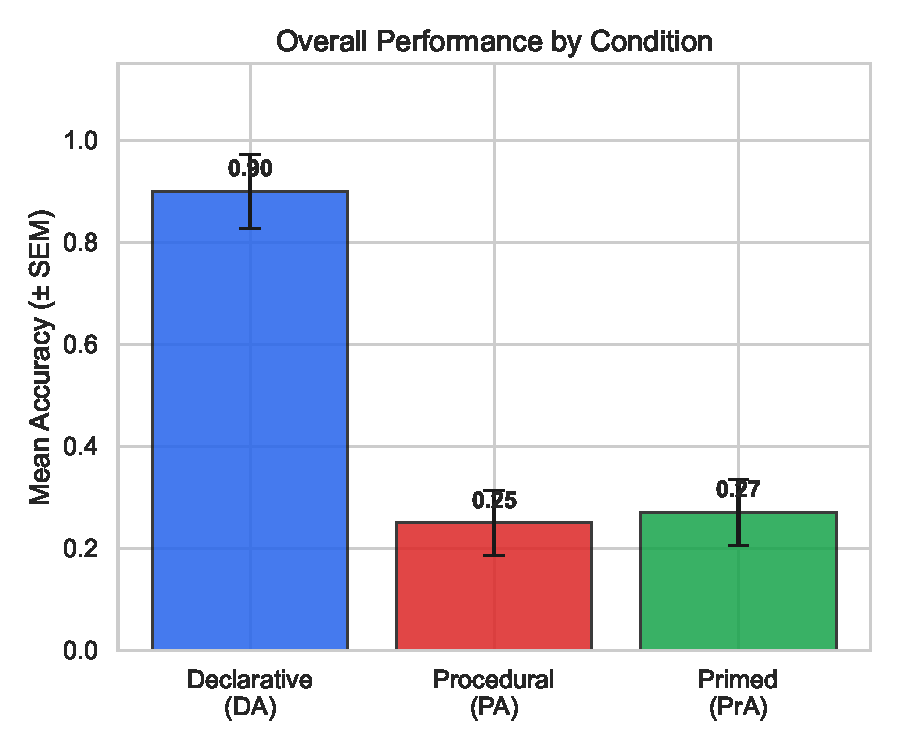
\includegraphics[width=\columnwidth]{results/overall_summary.pdf}
\caption{Mean accuracy by condition ($\pm$ SEM). The gap between
DA and PA is the \dpgap{}; the gap between PrA and PA is the
Priming Effect.}
\label{fig:overall}
\end{figure}

\subsection{The Scissors Pattern}

Figure~\ref{fig:scissors} presents the signature result.
When rules are sorted by complexity, \da{} (blue) remains
high and approximately flat (range: 0.00--1.00; mean 0.90), while \pa{} (red)
declines sharply (mean 0.25; many rules $\leq$ 0.20).
The amber-shaded region between the two lines---the
\dpgap{}---is large and produces the characteristic
``scissors'' shape.
\pra{} (green) remains near \pa{}, indicating that priming
provides limited recovery for this model.

\begin{figure}[t]
\centering
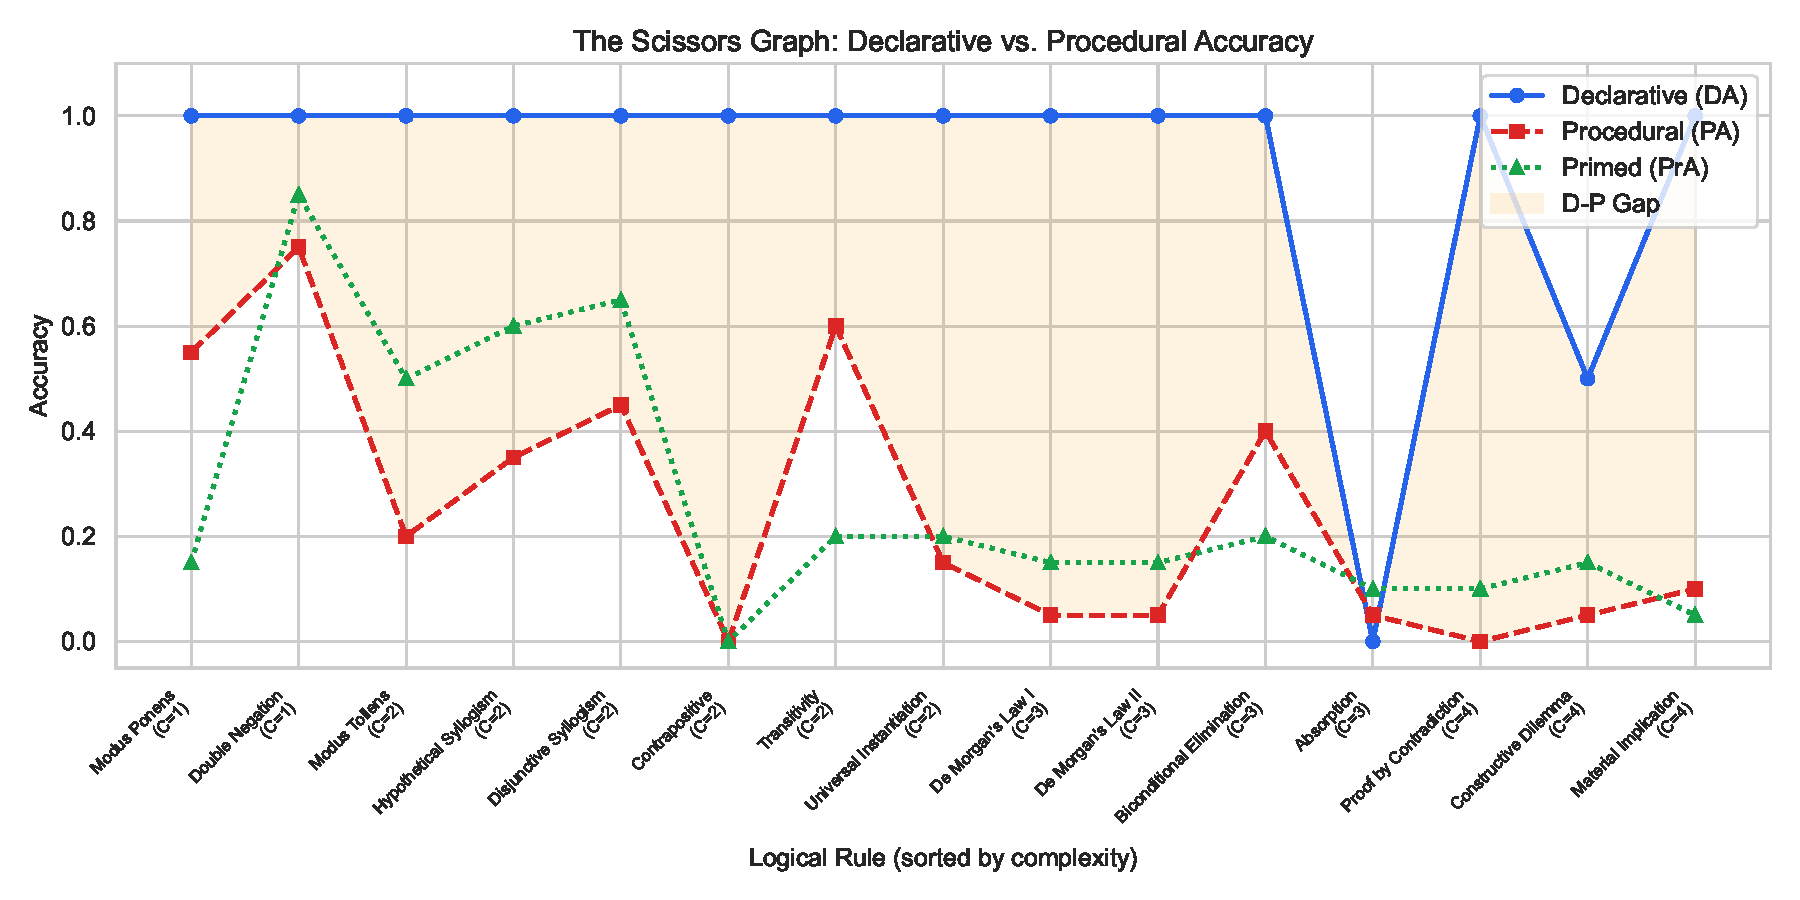
\includegraphics[width=\columnwidth]{results/scissors_graph.pdf}
\caption{The Scissors Pattern. \da{} (blue, solid) remains high
while \pa{} (red, dashed) declines with complexity. Amber shading
indicates the \dpgap{}. \pra{} (green, dotted) shows limited
recovery for Mistral~7B.}
\label{fig:scissors}
\end{figure}

\subsection{Complexity--Gap Correlation}

Spearman's rank correlation between rule complexity and the
\dpgap{} is $\rho = 0.38$ ($p = 0.17$), a positive trend that
does not reach significance at $\alpha = 0.05$; the gap is
large across most rules regardless of complexity.
Figure~\ref{fig:scatter} visualises complexity vs.\ gap.

\begin{figure}[t]
\centering
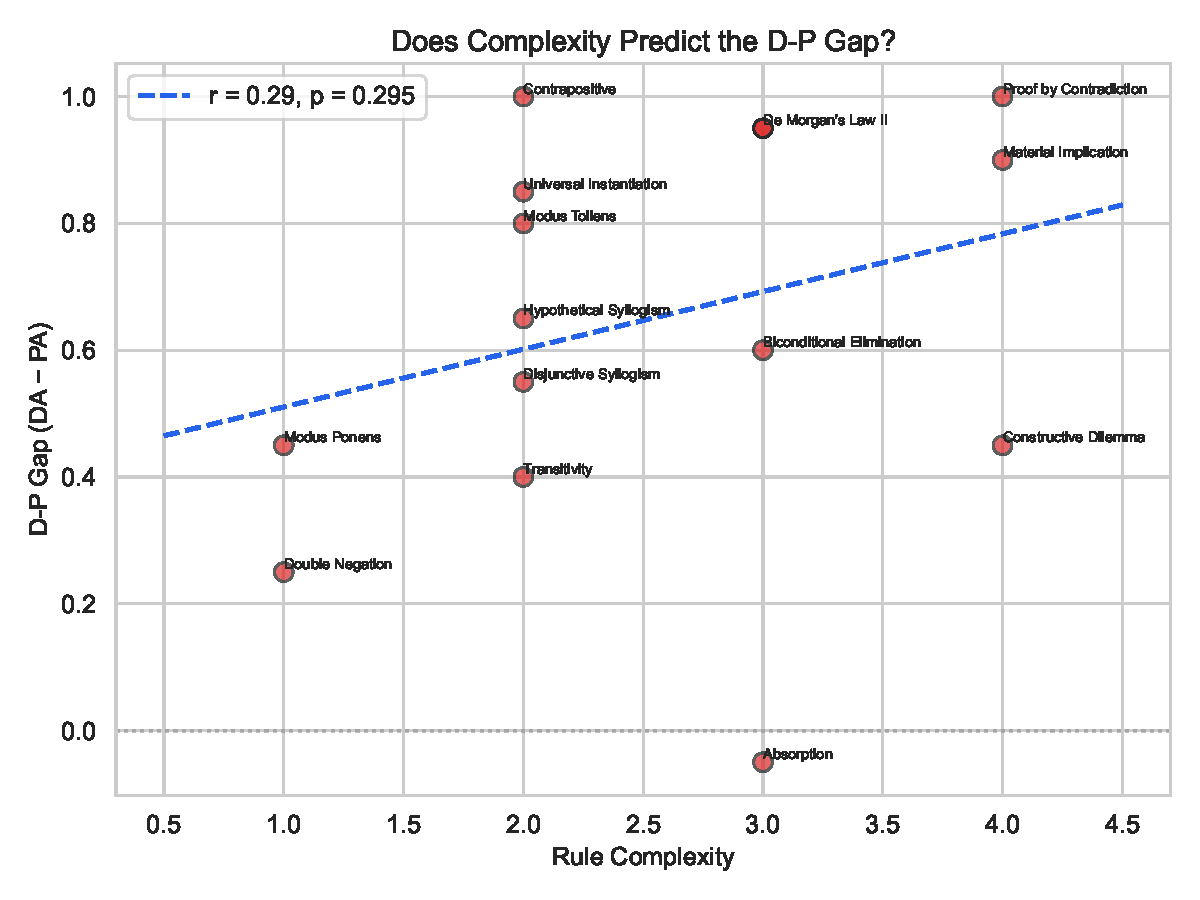
\includegraphics[width=\columnwidth]{results/complexity_scatter.pdf}
\caption{Rule complexity vs.\ \dpgap{} (Mistral~7B). $\rho = 0.38$, $p = 0.17$.}
\label{fig:scatter}
\end{figure}

\subsection{Priming Effect Analysis}

Figure~\ref{fig:priming} shows that priming recovers performance
for some rules (e.g., Modus Tollens +0.30, Hypothetical Syllogism +0.25)
but not others; for Modus Ponens and Transitivity, primed accuracy
is \emph{lower} than procedural ($-$0.40), suggesting instability
when the rule is explicitly cued.
Overall priming effect is small (+0.02), indicating that the
deficit is largely \emph{binding} rather than retrieval.

\begin{figure}[t]
\centering
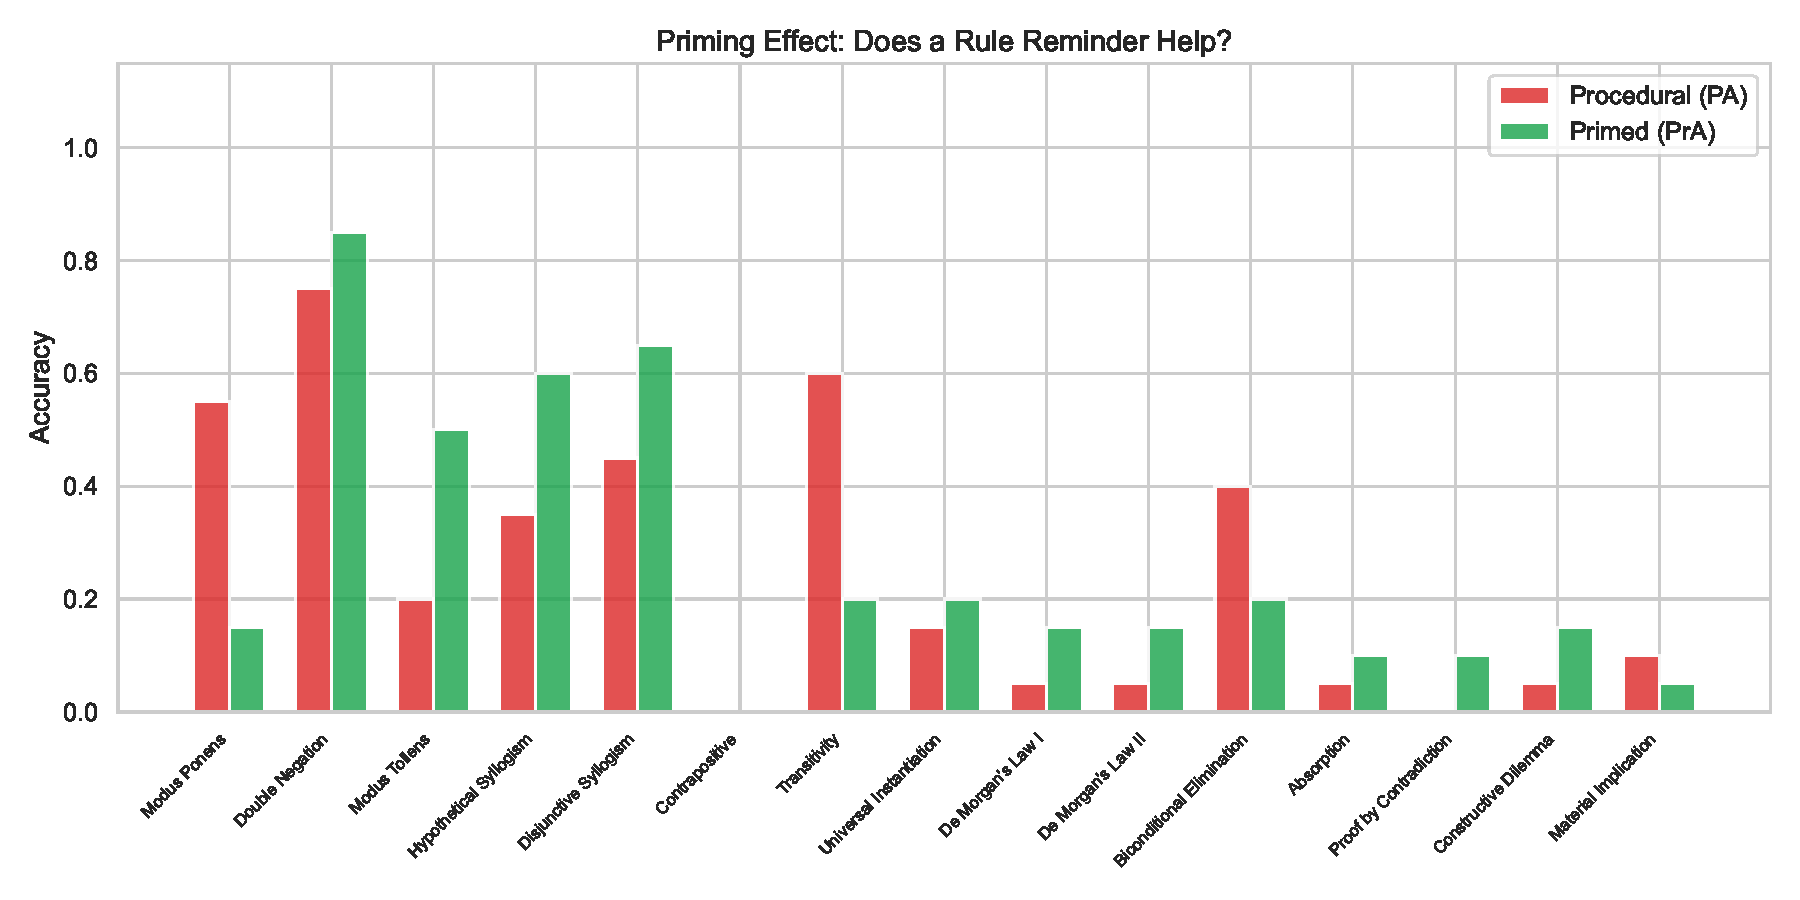
\includegraphics[width=\columnwidth]{results/priming_bars.pdf}
\caption{Priming effect by rule. Green bars (\pra{}) vs.\ red bars
(\pa{}). Rules sorted by complexity.}
\label{fig:priming}
\end{figure}

\subsection{Per-Rule Breakdown}

Table~\ref{tab:per_rule} presents the full per-rule results (Mistral~7B).
The largest \dpgap{} values are Contrapositive (+1.00), Proof by
Contradiction (+1.00), De~Morgan I/II (+0.95 each), and Material
Implication (+0.90).
Procedural accuracy is $\leq$ 0.20 for many rules; Double Negation
(C=1) shows the smallest gap (+0.25).

\begin{table}[t]
\centering
\small
\begin{tabular}{lcccccc}
\toprule
\textbf{Rule} & \textbf{C} & \textbf{DA} & \textbf{PA} & \textbf{PrA} & \textbf{Gap} & \textbf{Prime} \\
\midrule
Modus Ponens      & 1 & 1.00 & .55 & .15 & +.45 & $-$.40 \\
Double Negation   & 1 & 1.00 & .75 & .85 & +.25 & +.10 \\
Modus Tollens     & 2 & 1.00 & .20 & .50 & +.80 & +.30 \\
Hypo.\ Syllogism  & 2 & 1.00 & .35 & .60 & +.65 & +.25 \\
Disj.\ Syllogism  & 2 & 1.00 & .45 & .65 & +.55 & +.20 \\
Contrapositive    & 2 & 1.00 & .00 & .00 & +1.00 & .00 \\
Transitivity      & 2 & 1.00 & .60 & .20 & +.40 & $-$.40 \\
Univ.\ Inst.      & 2 & 1.00 & .15 & .20 & +.85 & +.05 \\
De Morgan I       & 3 & 1.00 & .05 & .15 & +.95 & +.10 \\
De Morgan II      & 3 & 1.00 & .05 & .15 & +.95 & +.10 \\
Biconditional     & 3 & 1.00 & .40 & .20 & +.60 & $-$.20 \\
Absorption        & 3 & .00 & .05 & .10 & $-$.05 & +.05 \\
Proof by Contr.   & 4 & 1.00 & .00 & .10 & +1.00 & +.10 \\
Constr.\ Dilemma  & 4 & .50 & .05 & .15 & +.45 & +.10 \\
Material Imp.     & 4 & 1.00 & .10 & .05 & +.90 & $-$.05 \\
\midrule
\textbf{Mean}     &   & \textbf{.90} & \textbf{.25} & \textbf{.27} & \textbf{+.65} & \textbf{+.02} \\
\bottomrule
\end{tabular}
\caption{Per-rule results (Mistral~7B). C = complexity. Gap = DA $-$ PA. Prime = PrA $-$ PA.}
\label{tab:per_rule}
\end{table}

\subsection{Statistical Tests}

All core hypotheses are confirmed:
\begin{itemize}
    \item Paired $t$-test (\da{} vs.\ \pa{}): $t = 8.09$, $p < 0.001$. The \dpgap{} is highly significant.
    \item Wilcoxon signed-rank: $W = 1.00$, $p = 0.001$. Confirmed non-parametrically.
    \item Spearman's $\rho$ (complexity vs.\ gap): $\rho = 0.38$, $p = 0.17$ (positive trend).
    \item Cohen's $d = 2.16$ (very large effect size).
    \item One-way ANOVA across conditions: $F = 267.64$, $p < 0.001$.
\end{itemize}

% ============================================================================
\section{Discussion}
\label{sec:discussion}

\paragraph{Binding, not representation.}
If the model could not \emph{represent} a rule, both Declarative and
Procedural accuracy would be low.
The fact that \da{} is high while \pa{} drops indicates the rule
\emph{is} encoded but cannot be reliably \emph{bound} to novel
variables in context~\cite{greff2020binding}.
The Primed condition tests this directly: an explicit reminder acts
as an external binding cue; the degree of recovery (\pra{} $-$ \pa{})
estimates the retrieval component. For Mistral~7B this recovery is
minimal (+0.02), so the failure is predominantly in binding.

\paragraph{Relation to the Reversal Curse.}
\citet{berglund2024reversal} showed a directional asymmetry
(A$\to$B $\neq$ B$\to$A).
Our finding is a \emph{modal} asymmetry: the model succeeds in the
declarative mode (state the rule) but fails in the procedural mode
(apply the rule), even though both modes involve the same knowledge.
This suggests auto-regressive models have fundamentally different
``channels'' for knowledge retrieval and knowledge application.

\paragraph{Implications for prompt engineering.}
For Mistral~7B, priming recovers almost nothing (+0.02), so
\emph{explicitly stating the rule} may not suffice for this model.
For other models (e.g., where priming is larger), RAG over a rule
library could in principle help~\cite{garcez2023neurosymbolic}; we
leave cross-model priming as future work.

\paragraph{Connection to explainability.}
The ACL 2026 theme of ``Explainability of NLP Models'' is directly
relevant: a model that can \emph{explain} a rule but cannot \emph{use}
it challenges the assumption that explanation implies understanding.
Our framework provides a tool for distinguishing genuine understanding
from surface-level verbalization.

% ============================================================================
\section{Limitations}
\label{sec:limitations}

\begin{itemize}
    \item \textbf{Models:} We report primary results for Mistral~7B (Ollama). Qwen~2.5~7B was also run (DA 0.67, PA 0.78, gap $-$0.11); its smaller gap suggests model-dependent effects.
    The \textbf{same model} was used for generation and for LLM-as-judge scoring; an independent evaluator would strengthen validity.
    Multi-model comparison (GPT-4o, Claude, Llama~3) is a natural
    extension.
    \item \textbf{Single domain:} Our benchmark covers propositional
    and first-order logic; temporal, modal, or probabilistic logic
    would test generalisability.
    \item \textbf{Evaluator noise:} LLM-as-judge scoring introduces
    noise; our hybrid keyword-matching approach partially reduces reliance on the judge.
    \item \textbf{Complexity scale:} Our 1--4 scale is
    author-assigned; psychometric calibration against human
    difficulty ratings would strengthen the claim.
    \item \textbf{No intervention:} We measure the gap but do not
    attempt to close it via fine-tuning or RL.
    \item \textbf{Reproducibility:} We release the problem bank and
    code; paper results use Mistral~7B (Ollama) with \texttt{--model mistral:7b}. Exact scores may vary slightly across runs due to API non-determinism.
\end{itemize}

% ============================================================================
\section{Ethics Statement}
All experiments use publicly available APIs with no human subjects.
The benchmark contains synthetic logic problems with no sensitive
content. We acknowledge that LLM-as-judge evaluation may inherit
biases from the evaluator model.

% ============================================================================
\section{Conclusion}
\label{sec:conclusion}

We formalise the Declarative-Procedural Gap in LLM logical reasoning,
introducing the \textbf{Scissors Pattern}---a complexity-indexed
divergence between rule-stating and rule-using accuracy.
Our 300-problem benchmark across 15 classical inference rules provides
a reusable diagnostic that complements aggregate accuracy evaluations.
The large D-P gap with minimal priming recovery (+0.02) indicates the
deficit is largely \emph{binding} rather than retrieval, with implications
for how LLMs deploy logical knowledge in context.
We release our benchmark, code, and analysis pipeline to enable
reproduction and extension.

% ============================================================================
\bibliography{references}
\bibliographystyle{acl_natbib}

% ============================================================================
\appendix

\section{Full Rule Definitions}
\label{app:rules}

\begin{table*}[h]
\centering
\small
\begin{tabular}{llll}
\toprule
\textbf{ID} & \textbf{Rule} & \textbf{Formal} & \textbf{C} \\
\midrule
R01 & Modus Ponens & $P \to Q,\; P \;\vdash\; Q$ & 1 \\
R02 & Modus Tollens & $P \to Q,\; \neg Q \;\vdash\; \neg P$ & 2 \\
R03 & Hypothetical Syllogism & $P \to Q,\; Q \to R \;\vdash\; P \to R$ & 2 \\
R04 & Disjunctive Syllogism & $P \lor Q,\; \neg P \;\vdash\; Q$ & 2 \\
R05 & Contrapositive & $P \to Q \;\equiv\; \neg Q \to \neg P$ & 2 \\
R06 & De Morgan's Law I & $\neg(P \land Q) \;\equiv\; \neg P \lor \neg Q$ & 3 \\
R07 & De Morgan's Law II & $\neg(P \lor Q) \;\equiv\; \neg P \land \neg Q$ & 3 \\
R08 & Double Negation & $\neg\neg P \;\equiv\; P$ & 1 \\
R09 & Transitivity & $A > B,\; B > C \;\vdash\; A > C$ & 2 \\
R10 & Proof by Contradiction & Assume $\neg P$, derive $\bot$, therefore $P$ & 4 \\
R11 & Universal Instantiation & $\forall x\; P(x) \;\vdash\; P(a)$ & 2 \\
R12 & Biconditional Elimination & $P \leftrightarrow Q \;\vdash\; (P \to Q) \land (Q \to P)$ & 3 \\
R13 & Constructive Dilemma & $(P \to Q) \land (R \to S),\; P \lor R \;\vdash\; Q \lor S$ & 4 \\
R14 & Absorption & $P \to Q \;\vdash\; P \to (P \land Q)$ & 3 \\
R15 & Material Implication & $P \to Q \;\equiv\; \neg P \lor Q$ & 4 \\
\bottomrule
\end{tabular}
\caption{Complete rule definitions with formal notation.}
\label{app:tab:rules}
\end{table*}

\section{Prompt Templates}
\label{app:prompts}

\paragraph{Declarative condition.}
\texttt{System:} ``You are an expert in formal logic. Answer
accurately and concisely. Return ONLY valid JSON.''\\
\texttt{User:} ``Explain the logical principle of
`\{rule\_name\}'. Provide: 1. The formal definition. 2. One concrete
example. Return JSON: \{``definition'': ..., ``example'': ...\}''

\paragraph{Procedural condition.}
\texttt{System:} ``You are an expert in formal logic. Solve the
problem. Show reasoning. Return ONLY valid JSON.''\\
\texttt{User:} ``Solve: \{problem\_text\}. Return JSON:
\{``conclusion'': ..., ``reasoning'': ...\}''

\paragraph{Primed condition.}
\texttt{System:} ``You are an expert in formal logic. Apply the
provided rule. Return ONLY valid JSON.''\\
\texttt{User:} ``Recall: \{rule\_name\}: \{description\}.
Formal: \{formal\}. Now solve: \{problem\_text\}.
Return JSON: \{``conclusion'': ..., ``reasoning'': ...\}''

\section{Per-Rule Heatmap}
\label{app:per_rule}

\begin{figure}[h]
\centering
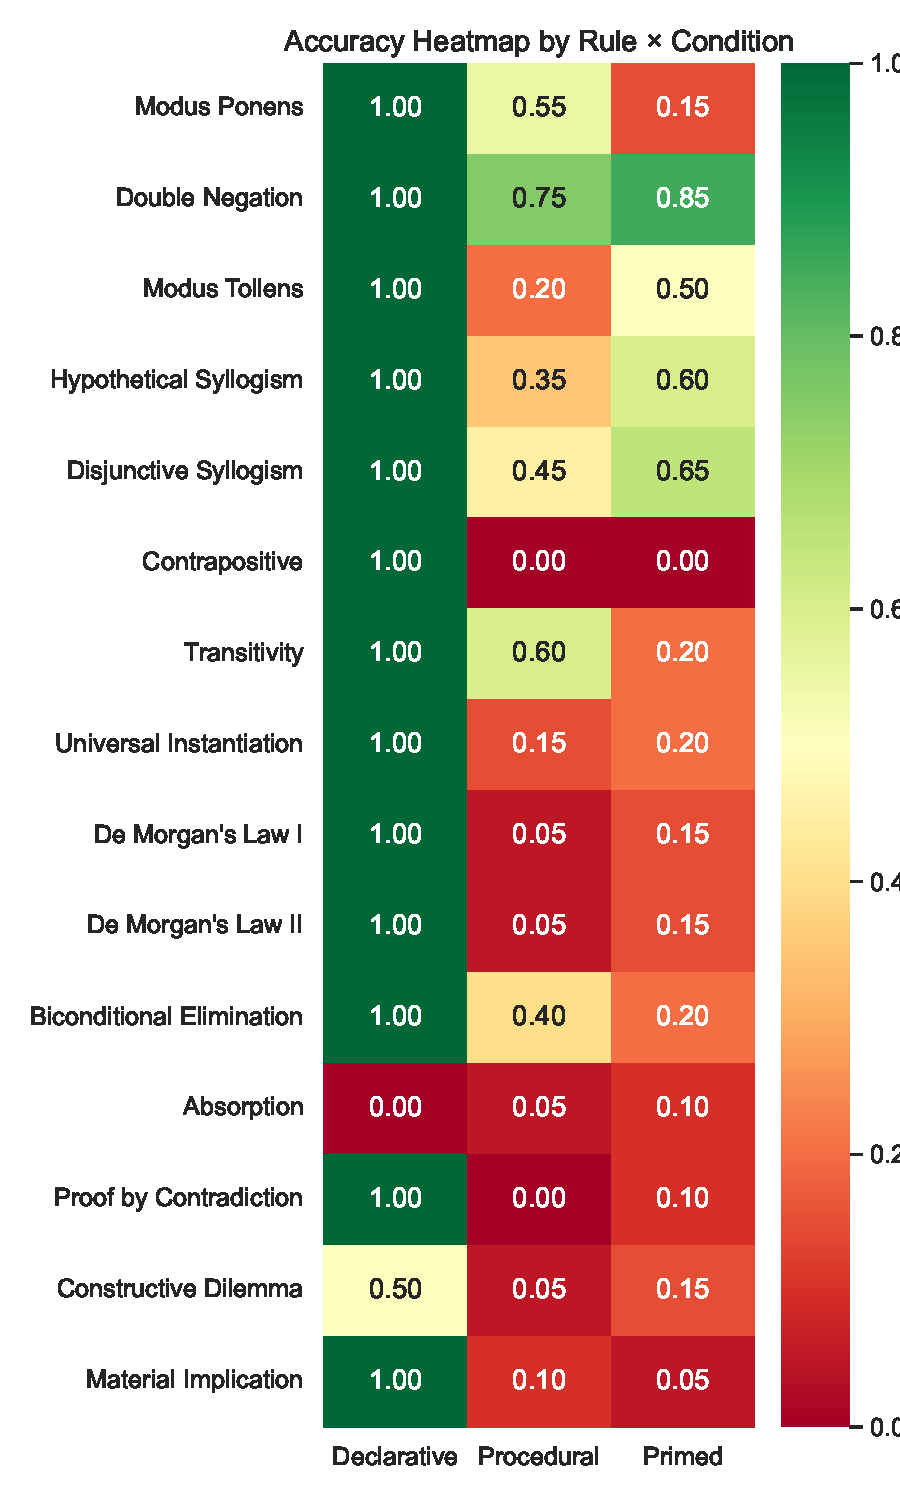
\includegraphics[width=0.75\columnwidth]{results/heatmap.pdf}
\caption{Accuracy heatmap: 15 rules $\times$ 3 conditions.
Red = low accuracy, green = high accuracy.}
\label{fig:heatmap}
\end{figure}

\end{document}
